\documentclass[14pt]{book}

\usepackage{fancyhdr}
\usepackage{graphicx}
\usepackage[margin=2.5cm]{geometry}
\usepackage{graphicx}
\usepackage{anysize}
\usepackage{xcolor}
\usepackage{caption}
\usepackage{subcaption}

\marginsize{2cm}{2cm}{2cm}{2cm} % Izquierda, derecha, arriba, abajo
\setlength{\parindent}{0cm}
\pagestyle{fancy}
\fancyhf{}
\fancyhead[L]{\footnotesize Redes de computadoras} %encabezado izquierda
\fancyhead[R]{\footnotesize David Pérez Jacome}   % derecha
\fancyfoot[L]{\footnotesize}  %izquierda
\fancyfoot[C]{Página \thepage}
\renewcommand{\footrulewidth}{0.4pt}

\begin{document}
\begin{center}
  \newcommand{\HRule}{\rule{\linewidth}{0.5mm}}
  \begin{minipage}{0.48\textwidth}
    \begin{flushleft}
      
\includegraphics[scale = 0.08]{images/logo_unam.png}
    \end{flushleft}
  \end{minipage}
  \begin{minipage}{0.48\textwidth}
    \begin{flushright}
      
\includegraphics[scale =0.22]{images/logo_ciencias.png}
    \end{flushright}
  \end{minipage}
  \vspace*{-1.5cm}
  \textsc{\huge Nacional Autónoma de México \\ \vspace{-4px} Universidad }\\[2cm]
  \textsc{\LARGE Facultad de Ciencias}\\[1.5cm]
  \begin{minipage}{0.9\textwidth}
    \begin{center}
      \textsc{\LARGE Redes de computadoras}
    \end{center}
  \end{minipage}\\[0.5cm]
  \vspace*{1cm}
  \HRule \\[0.4cm]
  { \huge \bfseries Practica 06}\\[0.4cm]
  \HRule \\[1.5cm]
  \begin{minipage}{0.52\textwidth}
    \begin{flushleft} \large \small \vspace{-0.6cm} \vspace{-0.6cm}
      Alumno David Pérez Jacome \\
    \end{flushleft}
  \end{minipage}
  \begin{minipage}{0.46\textwidth}
    \vspace{-0.6cm}
    \begin{flushright} \large \small \emph{Profesor:}
      Paulo Santiago de Jesús Contreras Flores \\
    \end{flushright}
  \end{minipage}
  \vspace*{1cm}
  \vspace{2cm}
  \begin{center}
    {\large 2023}
  \end{center}
\end{center}
\newpage

{\color{blue} \section*{\textbf{Practica 06}}}
\vspace{1em}

{\color{red} \subsection*{\textbf{Ruteo dinámico con RIPv2}}}
\vspace{1em}

{\color{red} \subsection*{\textbf{Objetivo}}}
\vspace{1em}

\begin{enumerate}
  \item El alumno aprenderá el uso del software de simulación de redes Packet Tracer.
  \item Configurará rutas dinámicas usando el protocolo RIP, en los router de diferentes redes.
  \item Configurará servidores DNS de diferentes dominios para que se comuniquen entre ellos.
\end{enumerate}

{\color{red} \subsection*{\textbf{Introducción}}}
\vspace{1em}

El Routing Information Protocol \textbf{(RIP)} es un protocolo de enrutamiento dinámico que utiliza el
recuento de saltos como métrica de enrutamiento para encontrar la mejor ruta entre la red de
origen y la de destino. Funciona en la capa de aplicación del modelo OSI y utiliza el puerto 520.
Es uno de los protocolos de enrutamiento más viejos, lo que conlleva a que se utilice en redes que
se conforman por dispositivos antiguos.\\

El recuento de saltos equivale al número de routers por los que tenga que pasar la información
entre la red de origen y la de destino. De esto se concluye que la ruta con el menor número de saltos
es la mejor ruta para llegar a una red, por lo que se coloca en la tabla de enrutamiento. Pero como
todo protocolo tiene un limite en la cantidad de saltos que pueden existir para alcanzar una red,
el recuento de saltos máximo permitido es 15; si en una ruta hubiera un recuento de 16 saltos (o
más) se considerará que al red es inalcanzable. Gracias a esto RIP evita los bucles de enrutamiento
en la ruta.\\

RIP envia las actualizaciones de la red cada 30 segundos. Lo importante aqui es que estas
actualizaciones se envian a todos los componentes de la red en la que se ha configurado el protocolo;
es decir, se realiza por medio de un broadcast.\\

Finalmente, recapitulemos cuales son las principales caracteristicas de este protocolo:\\

\begin{enumerate}
  \item Las actualizaciones (información de enrutamiento) de la red se intercambian periódicamente.
  \item Las actualizaciones siempre se transmiten por medio de un broadcast.
  \item Siempre se envian las tablas de enrutamiento completas en las actualizaciones.
  \item Los routers siempre confían en la información de enrutamiento recibida de sus routers vecinos.
\end{enumerate}

\vspace{2em}

{\color{red} \subsection*{\textbf{Desarrollo}}}
\vspace{1em}

Para comenzar esta practica vamos a configurar nuevas infraestructuras, una para la red de Google:\\

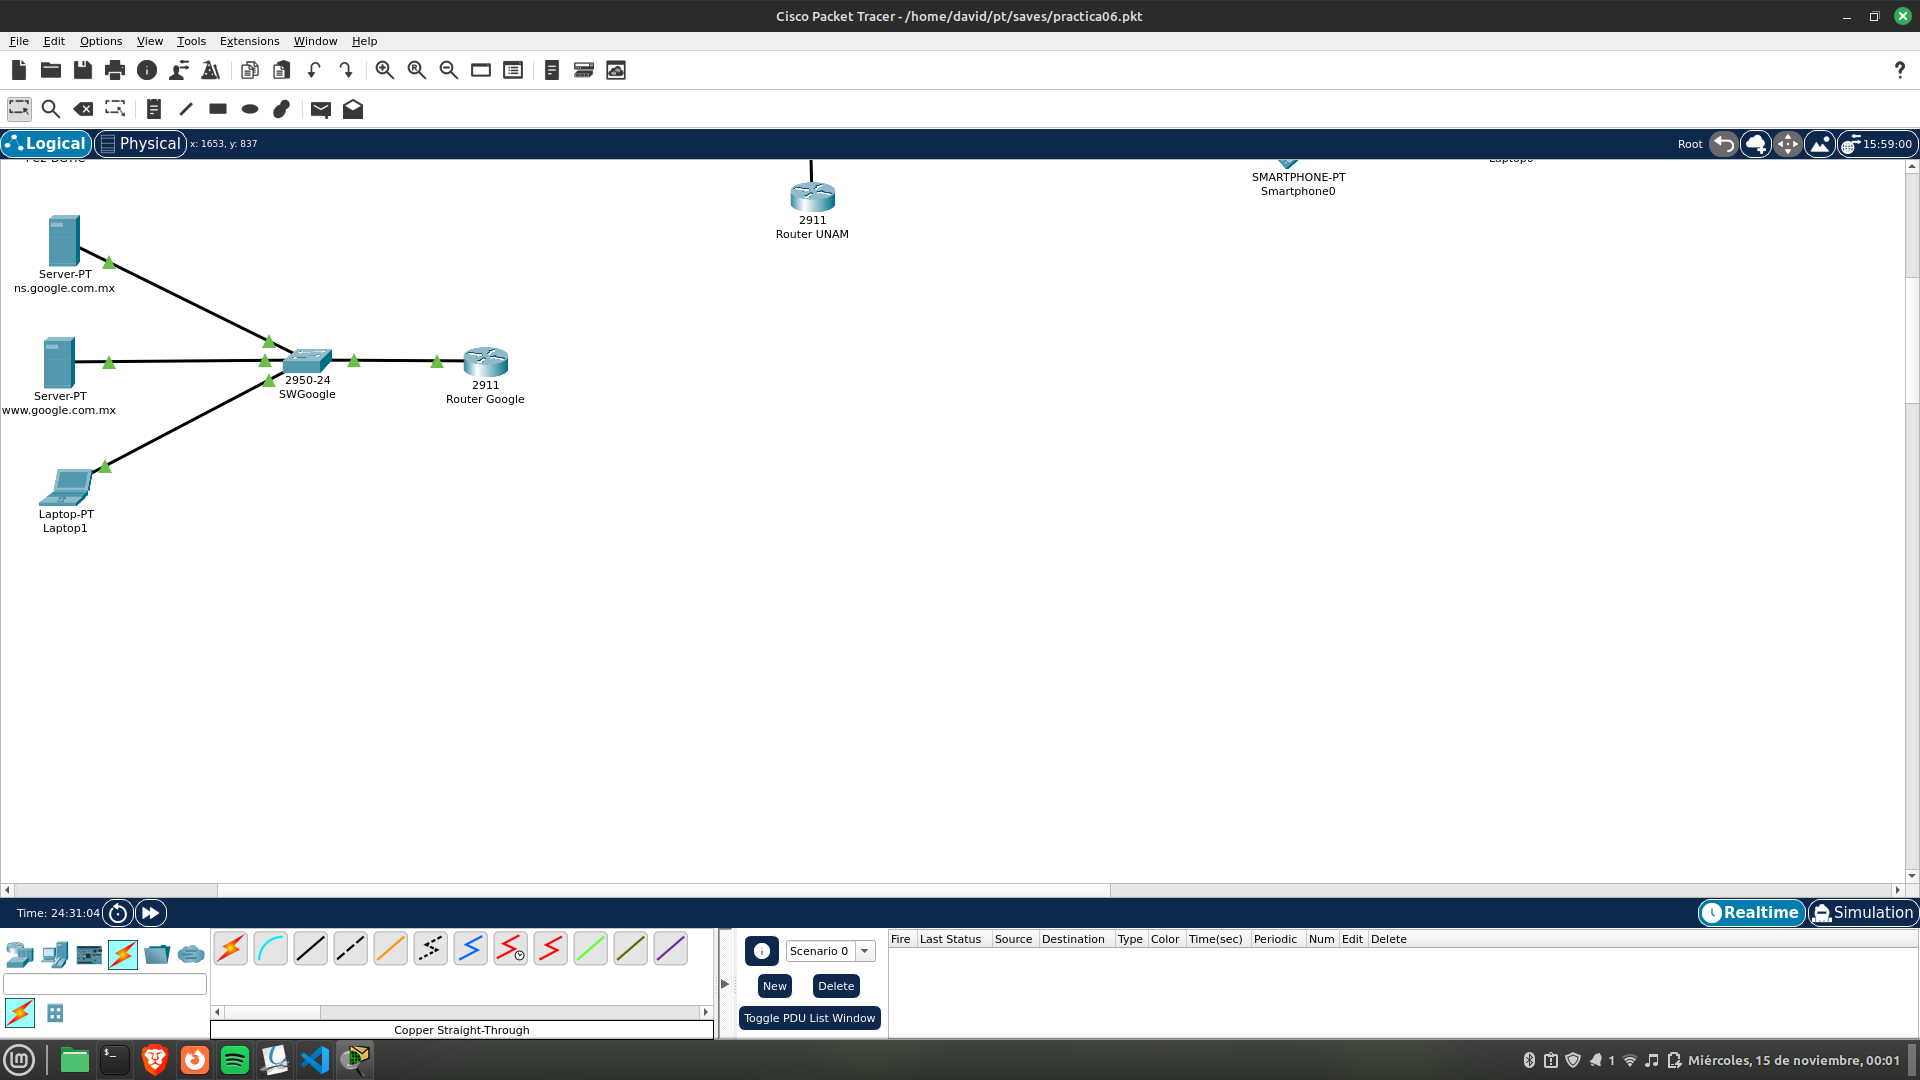
\includegraphics[width=12cm, height=8cm]{images/redgoogle.png}\\

Otra para la red de Telmex-Infinitum:\\

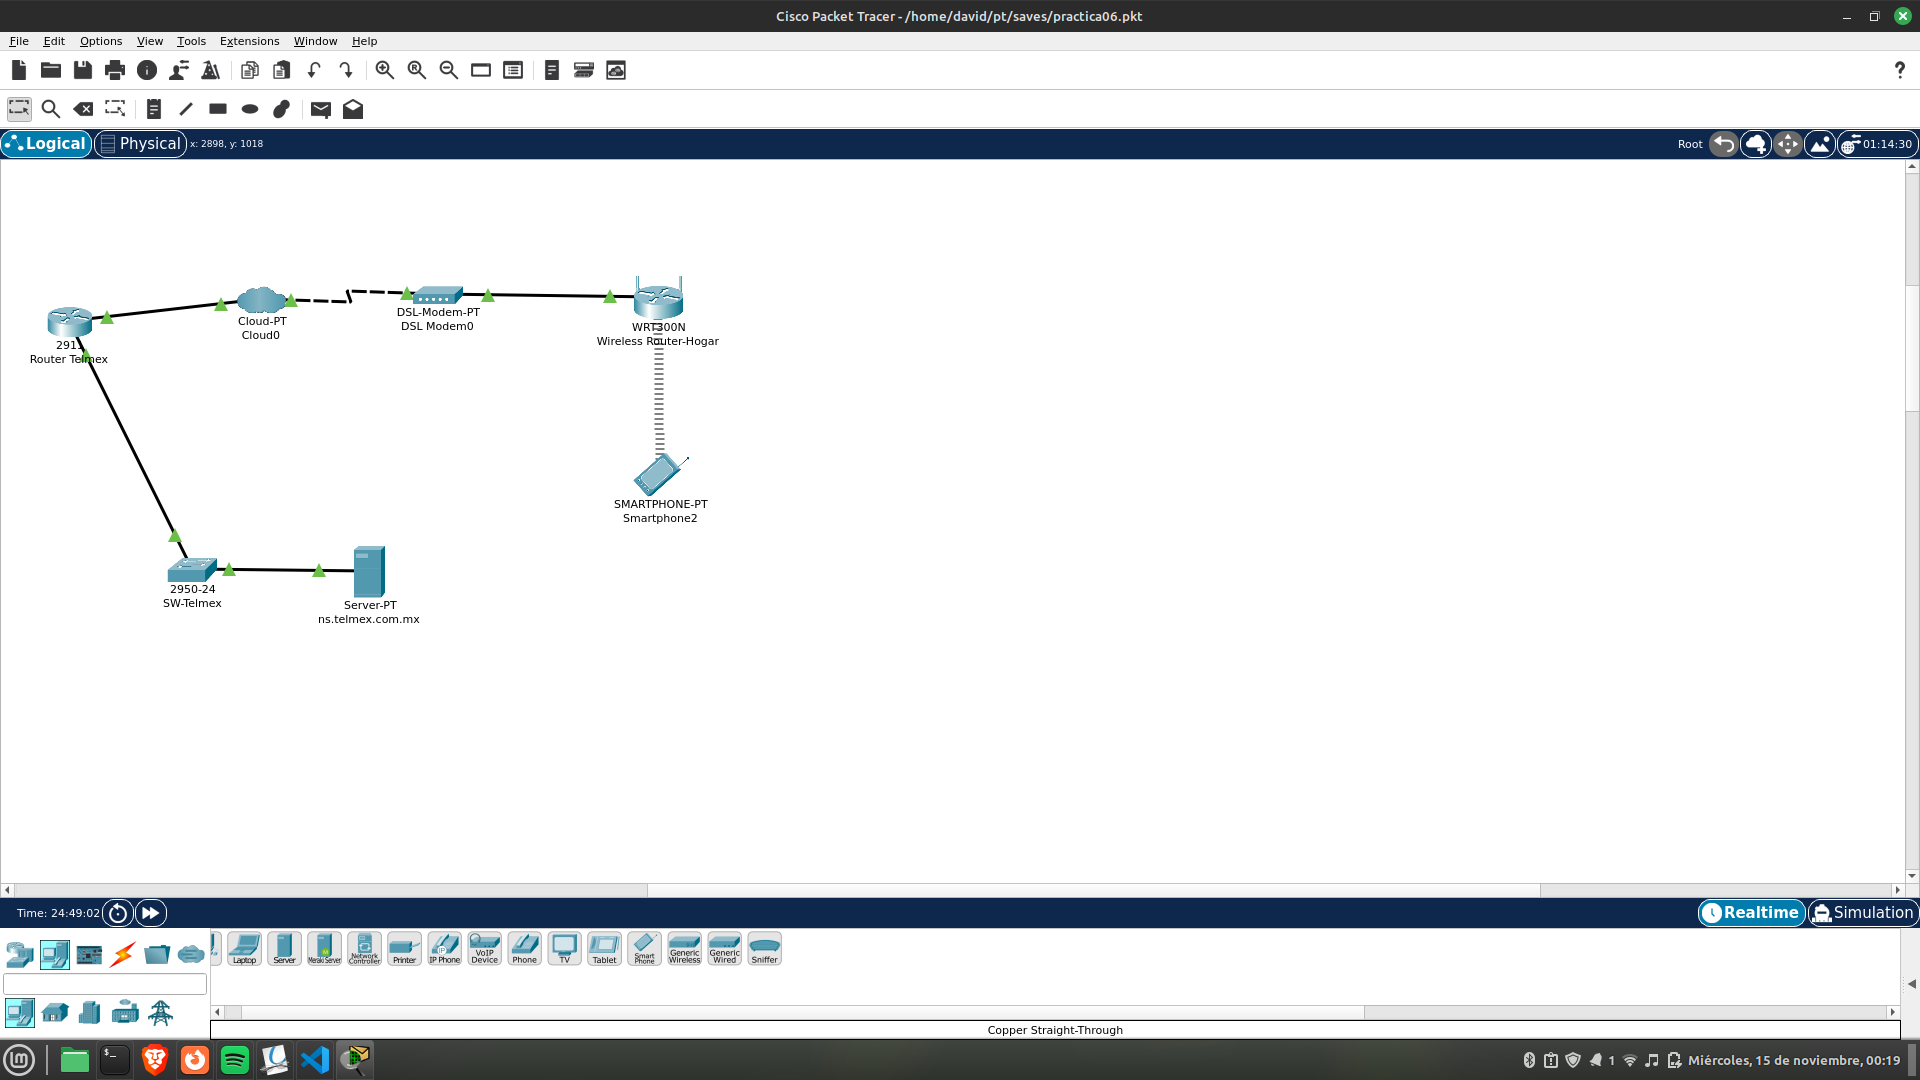
\includegraphics[width=12cm, height=8cm]{images/telmexred.png}\\

Por ahora solamente me guie de las capturas iniciales del pdf para mostrar las capturas anteriores, ahora vamos a configurar los respectivos dispositivos, iniciando con la red de Google MX.\\

Para iniciar vamos a configurar \textbf{ns.google.com.mx}, que es un servidor DNS asi que usamos las configuraciones correspondientes como activar el apartado de DNS, y desactivar HTTP, HTTPS. ademas de que como antes mencione ya habia agregado la IP y habia hecho las conexiones,
solamente tuve que configurar en los 3 dispositivos, el Gateway y DNS-Server como se muestra a continuación:\\

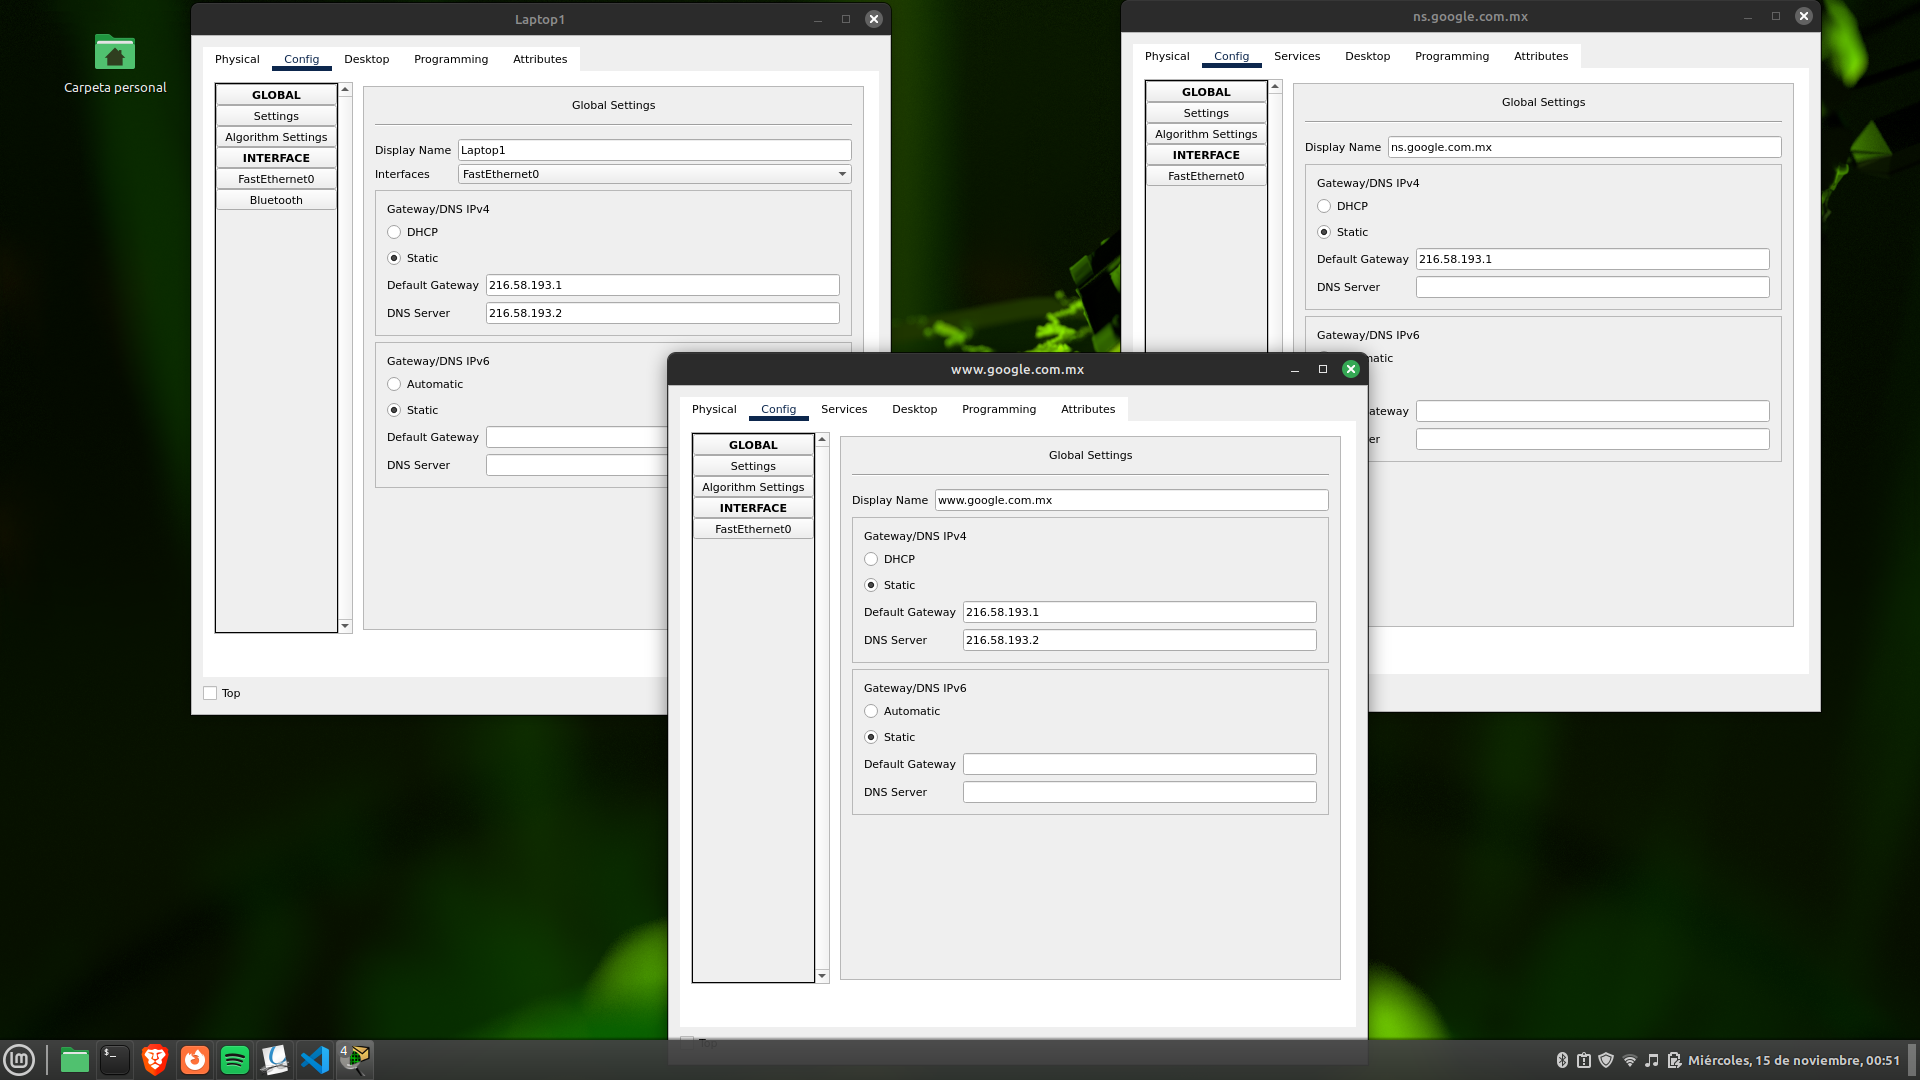
\includegraphics[width=12cm, height=8cm]{images/dnsconfiguaracion.png}\\

De igual manera configuramos el \textbf{ns.telmex.com.mx}:\\

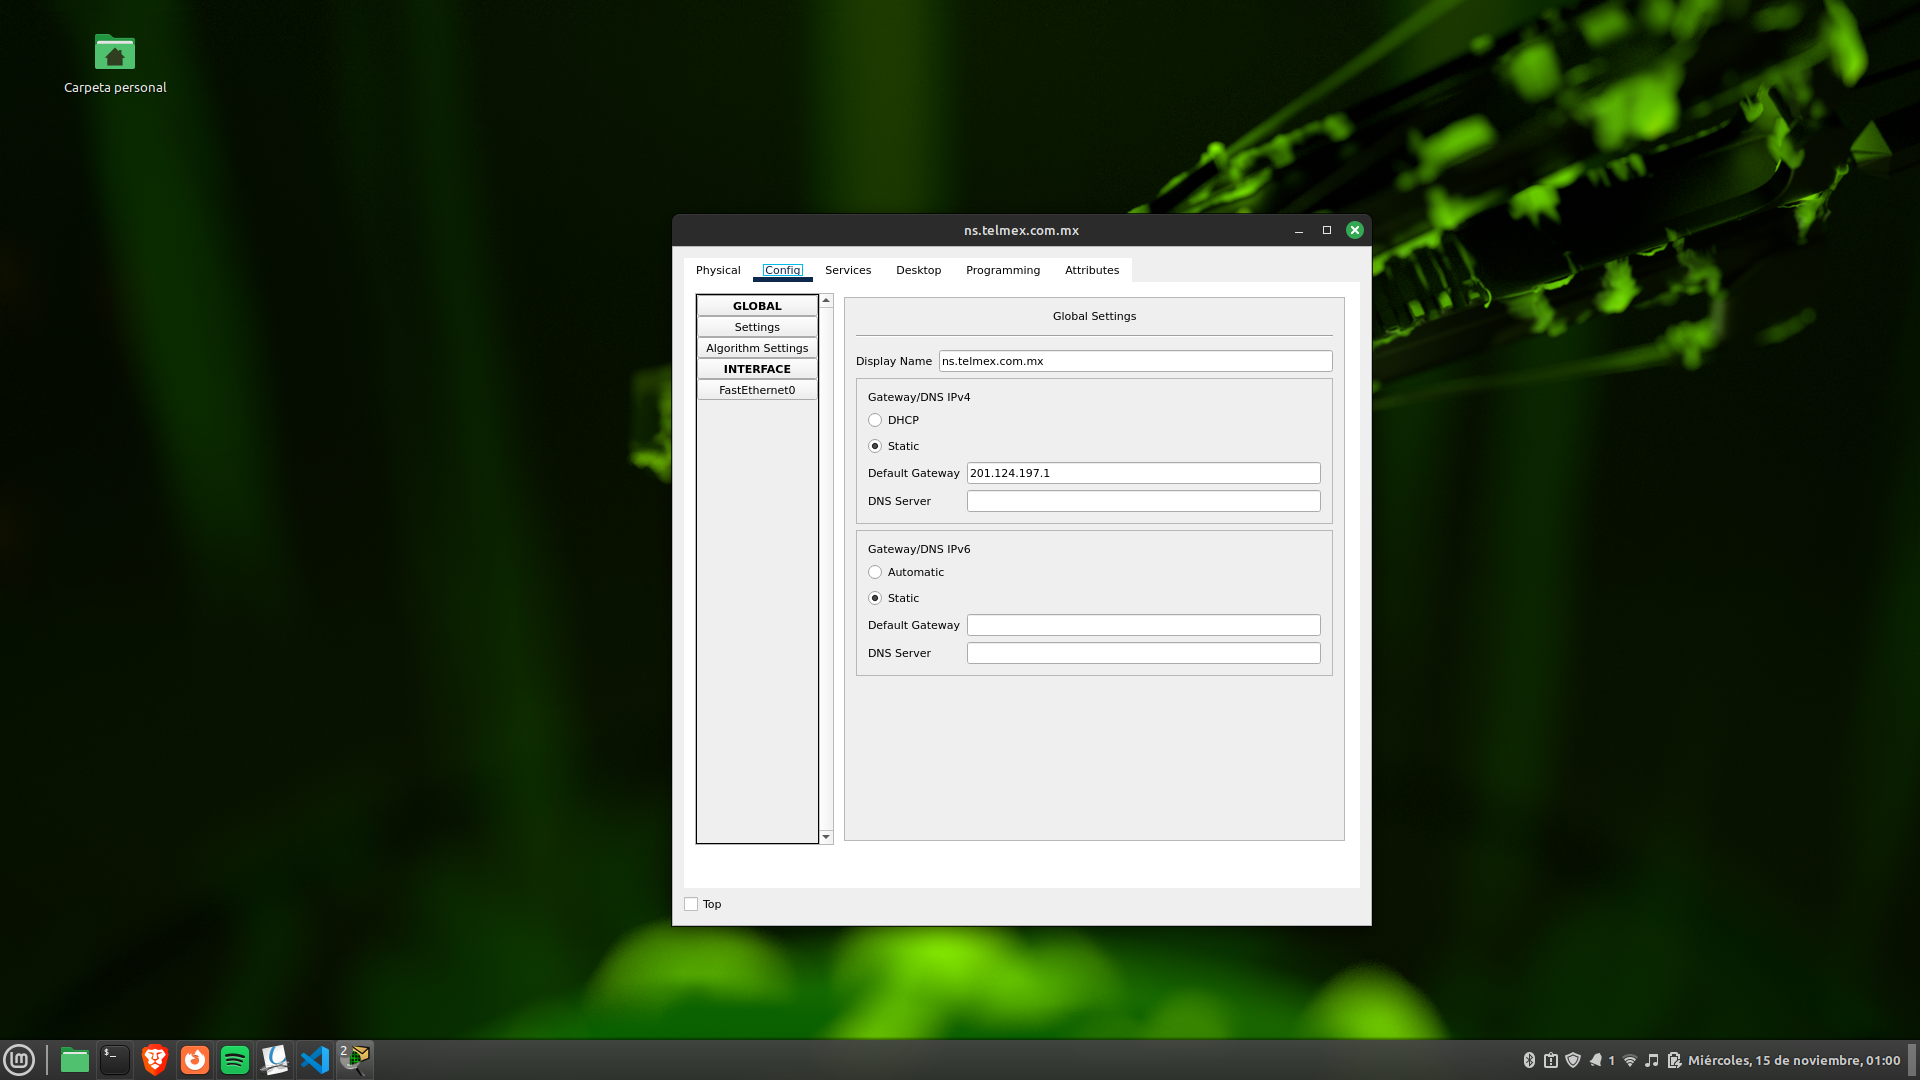
\includegraphics[width=12cm, height=8cm]{images/dnstelmex.png}\\

Ahora vamos a configurar el \textbf{Wireless Router-Hogar} similar a como lo configuramos el \textbf{RIU} más lo que nos especifica la tabla de las intrucciones del pdf.\\

Iniciamos con el \textbf{Internet Setup y Network Setup}:\\

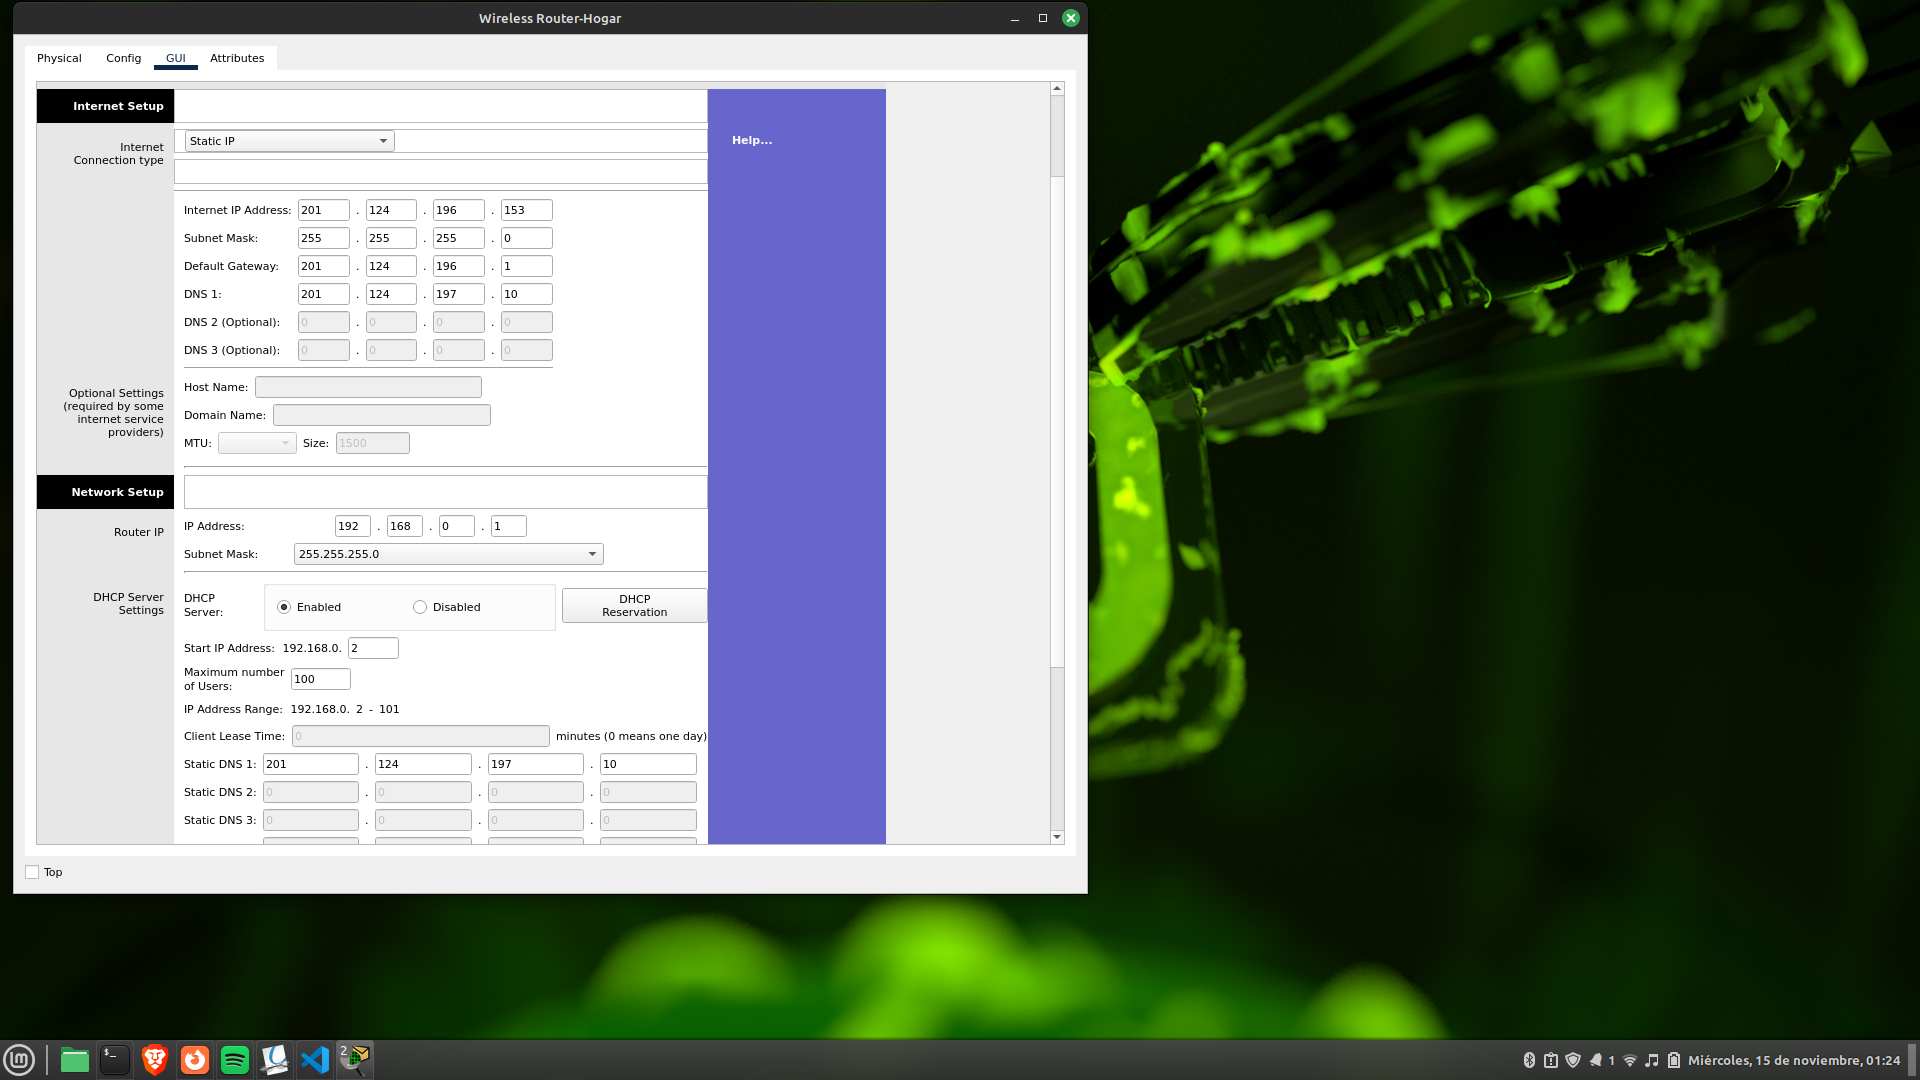
\includegraphics[width=12cm, height=8cm]{images/confiwireles.png}\\

Ahora \textbf{Basic Wireless Settings} simplemente menciono que le cambiamos el nombre a \textsf{Infinitum5678}.\\











\end{document}